\documentclass[
    a4paper,
    man,
    british
]{apa6}

\usepackage[british]{babel}
\usepackage[utf8]{inputenc}
\usepackage{epstopdf}
\usepackage{csquotes}
\usepackage[hidelinks]{hyperref}
\usepackage[
    style=apa,
    backend=biber,
    sortcites=true,
    sorting=nyt,
%    isbn=false,
%    url=false,
%    doi=false,
%    eprint=false,
    hyperref=false,
    backref=false,
%    firstinits=false,
]{biblatex}

\DeclareLanguageMapping{british}{british-apa}

% maps apacite commands to biblatex commands
\let \citeNP \cite
\let \citeA \textcite
\let \cite \parencite

%%%
% Apa Bib - enable reprint according to apa
%%%

% http://tex.stackexchange.com/questions/139805/how-to-differentiate-between-translated-and-reprinted-work-with-apa-style

\renewbibmacro*{related:reprintfrom}[1]{%
  \entrydata*{#1}{%
    \printtext{\mkbibemph{\printfield[apacase]{title}}}%
    \setunit{\bibpagespunct}%
    \printfield{pages}%
    \setunit{\addcomma\addspace}%
    \bibstring{byauthor}\addspace
    \printnames[apanames][-\value{listtotal}]{editor}%
    \ifnameundef{editor}
      {}
      {\addcomma\addspace
       \usebibmacro{apaeditorstrg}{editor}}
    \printnames[apanames][-\value{listtotal}]{author}%
    \setunit{\addcomma\addspace}%
    \usebibmacro{date}%
    \setunit{\addcomma\addspace}%
    \usebibmacro{location+publisher}%
    \newunit\newblock
    \usebibmacro{related}}}


\DefineBibliographyStrings{british}{
  reprintfrom = {Reprinted from}
}


\bibliography{bibliography}


%%%%%%%%%%%%%%%%%%%%%%%%%%%%%%%%%%%%%%%%%%%%%%%%%%%

\title{Some Long Sample Title : How APA can be used}
\shorttitle{Some Short Sample Title}
\author{Max Mustermann}
\affiliation{Some university}

\keywords{petri net, recall, long term working memory, expert domain knowledge}

\begin{document}

\maketitle

\section{Petri Nets as a Visual Modeling Language}

Petri nets are used to model systems by means of a graphical language\parencites(cf.)(){reisig2013understanding}.
In specific, in this study the Petri nets are aimed to be lay-outed similar to \citetitle{reisig2013understanding} \cite{reisig2013understanding}.



\printbibliography

\appendix

\section{Visual vocabulary of an Elementary System Net}
\label{app:elsysnet}

\begin{figure}
    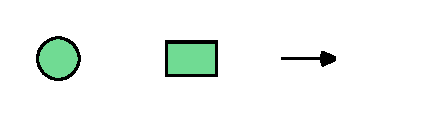
\includegraphics[scale=1]{graphics/visual_vocabulary_elementary_system_net}
    \caption{A circle depicts a place, a rectangle depicts a transition and an arrow depicts and arc. The arrow connects places with transitions and can be bent for that purpose. The green color is the standard color of the }
    \label{fig:visual_vocabulary_elementary_system_net}
\end{figure}


\end{document}
